\begin{figure}[h!]
    \begin{center}
    \caption{Effects on Ambulatorial Production}\label{fig:15}
    \begin{subfigure}{0.32\textwidth}
        \centering
        \caption{\scriptsize Total}\label{fig:15a}
        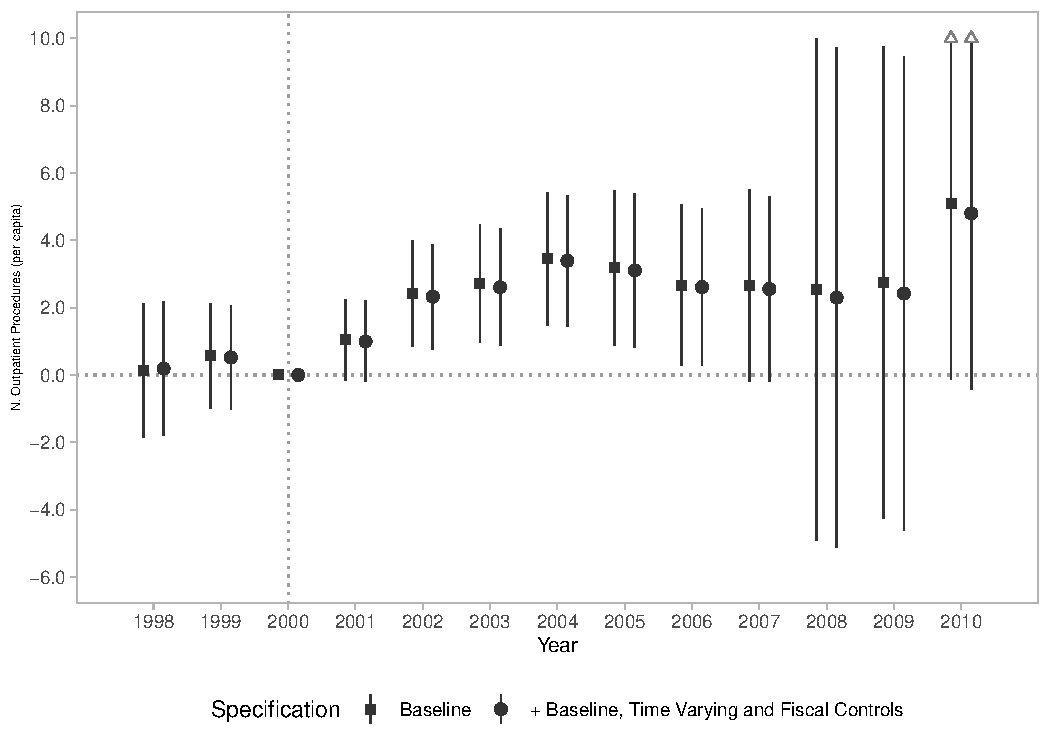
\includegraphics[width=\textwidth]{plots/sia_pcapita_dist_ec29_baseline_dist_ec29_baseline_15.pdf}
    \end{subfigure}
    \begin{subfigure}{0.32\textwidth}
        \centering
        \caption{\scriptsize Primary Care}\label{fig:15b}
        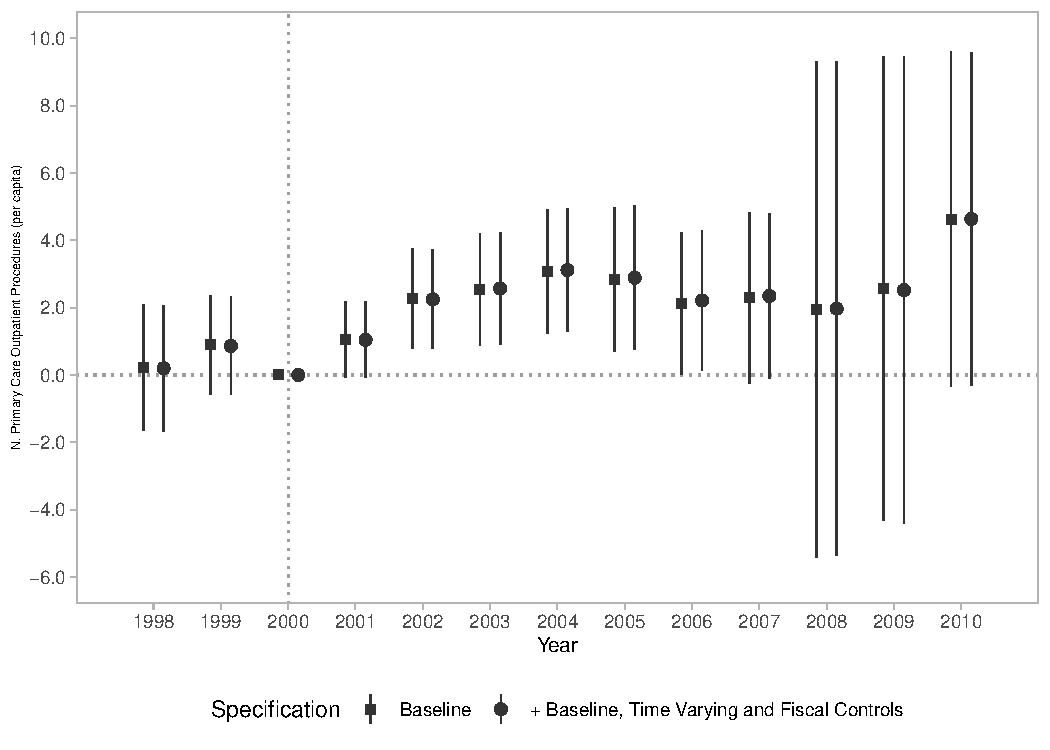
\includegraphics[width=\textwidth]{plots/sia_ab_pcapita_dist_ec29_baseline_dist_ec29_baseline_15.pdf}
    \end{subfigure}
    \begin{subfigure}{0.32\textwidth}
        \centering
        \caption{\scriptsize Low and Mid Complexity}\label{fig:15c}
        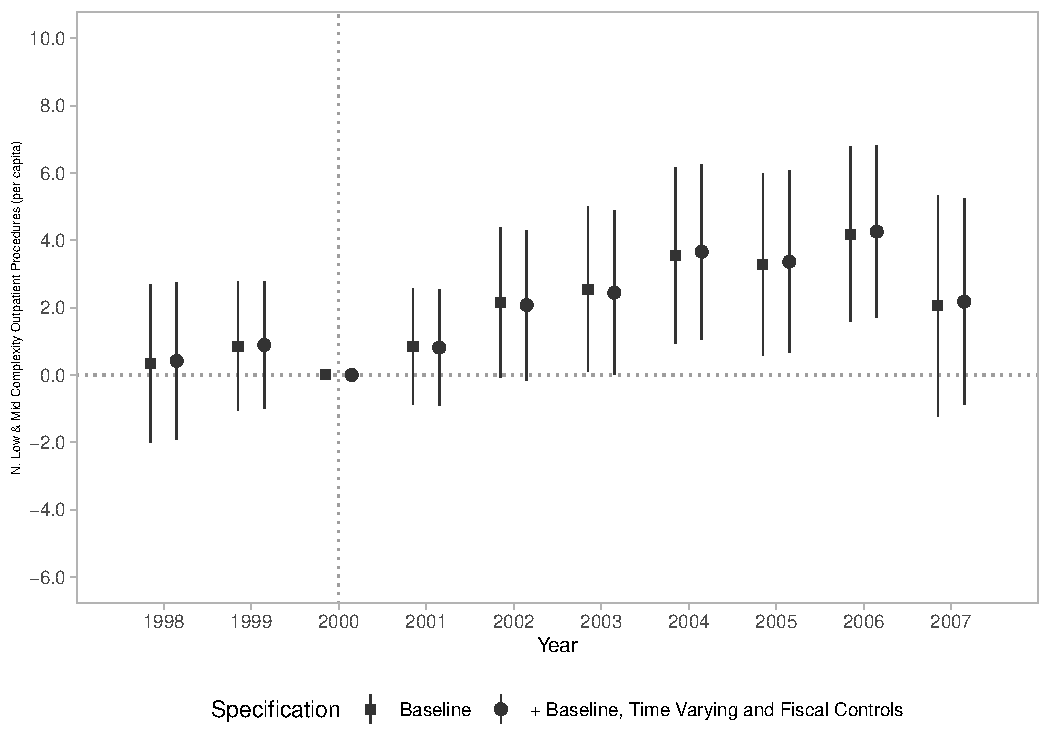
\includegraphics[width=\textwidth]{plots/sia_nprod_amb_lc_mun_pcapita_dist_ec29_baseline_dist_ec29_baseline_15.pdf}
    \end{subfigure}
    \begin{subfigure}{0.32\textwidth}
        \centering
        \caption{\scriptsize High Complexity}\label{fig:15d}
        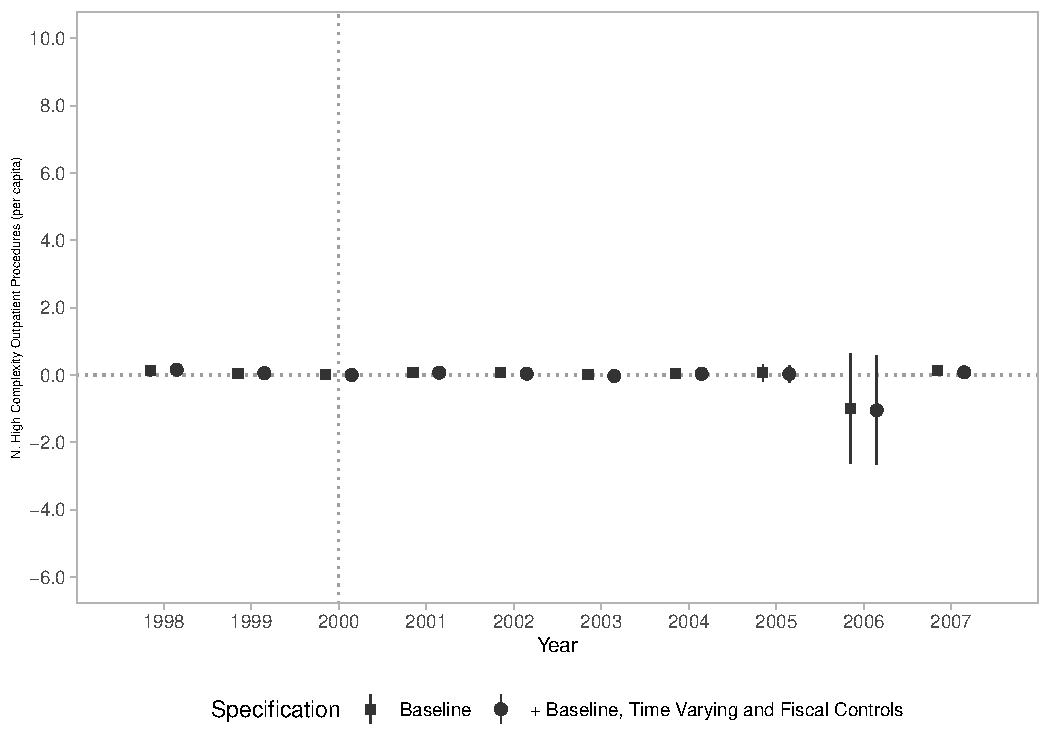
\includegraphics[width=\textwidth]{plots/sia_nprod_amb_hc_mun_pcapita_dist_ec29_baseline_dist_ec29_baseline_15.pdf}
    \end{subfigure}
    \begin{subfigure}{0.32\textwidth}
        \centering
        \caption{\scriptsize Performed by Low Skilled Worker}\label{fig:15e}
        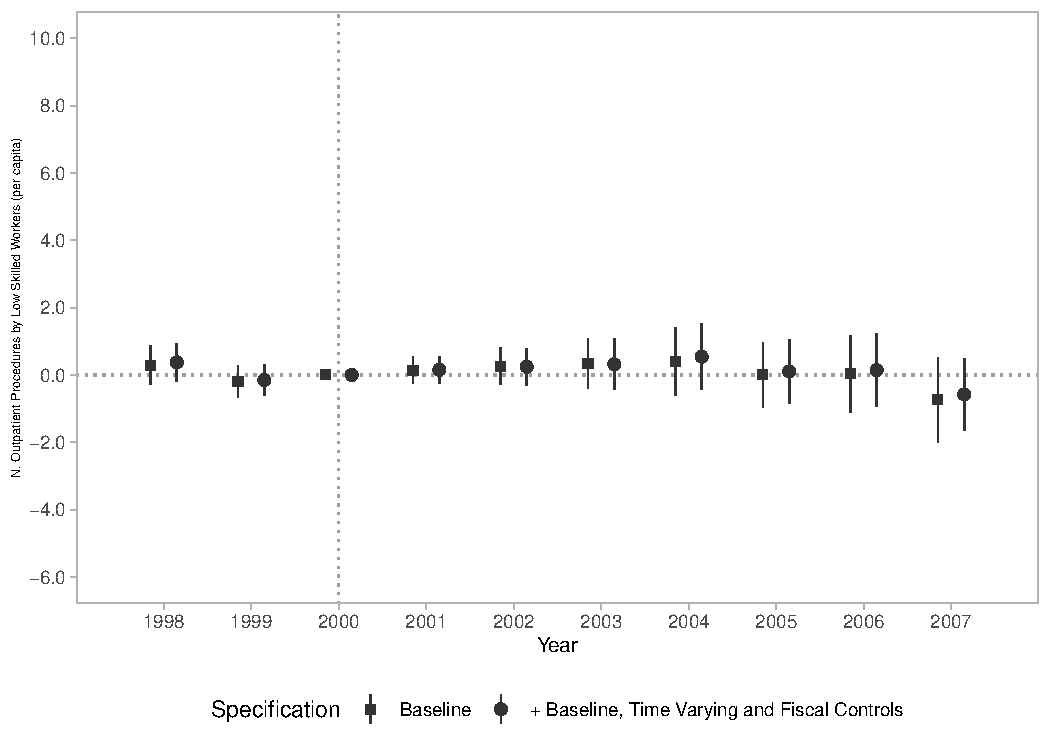
\includegraphics[width=\textwidth]{plots/sia_nprod_low_skill_mun_pcapita_dist_ec29_baseline_dist_ec29_baseline_15.pdf}
    \end{subfigure}
    \begin{subfigure}{0.32\textwidth}
        \centering
        \caption{\scriptsize Performed by High Skilled Worker}\label{fig:15f}
        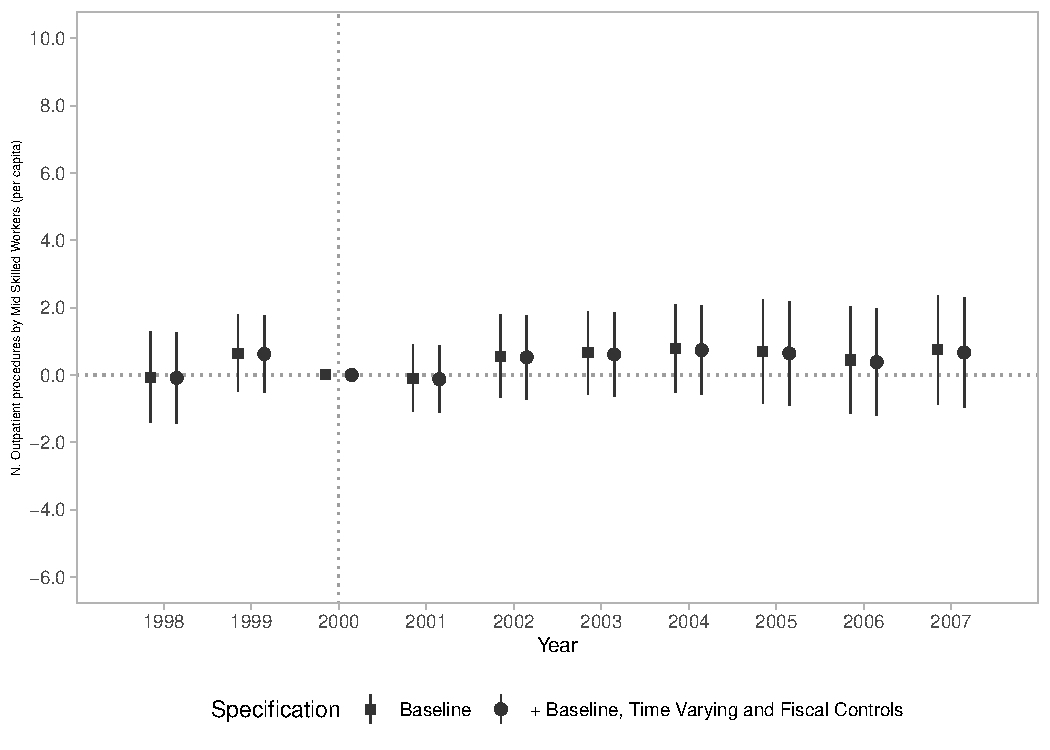
\includegraphics[width=\textwidth]{plots/sia_nprod_med_skill_mun_pcapita_dist_ec29_baseline_dist_ec29_baseline_15.pdf}
    \end{subfigure}
    
    \end{center}
    
        \scriptsize{Notes: The number of observations is 64710 for \ref{fig:15a} and \ref{fig:15b}, 49080 for the remaining. DiD Estimates from Equation \ref{eq:2}. Independent variable is the distance to the EC/29 target in p.p. Square dots represent the baseline model with municipality and state-year fixed effects. Round dots represent fully saturated specification (Column 4 in regression Tables). Lines represent 95\% confidence intervals. Arrows, when present, indicate confidence intervals out of the plot bounds. Standard errors are clustered in the municipality level.}
    
\end{figure}